 \chapter{浮游动物图像特征提取}

\section{特征提取方法}
\label{3.1}

图像特征提取是进行图像分析与图像识别的前提,可以通过这种方式对图像数据进行抽象和描述,给定一幅图像,我们只能得到一个$M \times N$的数据矩阵,而总结不出任何有效的信息,所以我们有必要对这个数据矩阵进行一定的处理,从而提取出有用的信息,方便我们作出对图像的描述。

在本节中,我们主要整理了图像处理领域的常用特征和网上分类、识别竞赛排名较为靠前的算法中用到的一些经典特征。

\subsection{图像处理领域常用特征}

\begin{enumerate}

\item 边界的周长:轮廓边界的周长,对轮廓边缘上的像素点进行统计。

\item 边界的曲率:表示目标物体边缘轮廓曲线的弯曲程度。

\item 面积:描述区域大小的特征,对区域内总像素点的数目进行统计。

\item 宽度和高度:最小外接矩形的宽度和高度。

\item 矩形度:表示目标物体的整个边缘轮廓在其最小外接矩形中的充满程度,当目标的轮廓形状越接近矩形时,矩形度的值越接近1。
    \begin{align}
    R=\frac{A}{WH}
    \end{align}
    其中,A为目标的面积,W、H分别为最小外接矩形的宽度和高度。

\item 体态比:目标最小外接矩形的长与宽的比值。
    \begin{align}
    C=\frac{W}{H}
    \end{align}
    
\item 圆形性:用目标区域的所有边界点定义的特征向量。
    \begin{align}
    C_{I}=\frac{\mu_{R}}{\sigma_{R}}
    \end{align}
    $\mu_{R}$为区域重心到边界点的平均距离,$\sigma_{R}$为从区域重心到边界点的距离的平均方差。

\item 偏心率:在一定程度上反映了物体轮廓形状与理想圆环的偏离。定义为焦点间距离$p$与长轴$q$的比值。
    \begin{align}
    E=\frac{p}{q}
    \end{align}
    
\item 凸率:表征物体边界轮廓的不规则程度,为目标区域面积与目标区域凸包面积两者的比值。
    \begin{align}
    C_{R}=\frac{A}{\sum_{x=1}^{M}\sum_{y=1}^{N}k(x,y)}
    \end{align}
    分母为凸包区域的面积。
    
\item 密集度:表示目标物体围成的区域的密集程度。
    \begin{align}
    C = \frac{A}{P^2}
    \end{align}
    $A$表示物体区域的面积,$L$表示物体轮廓的周长。圆形是所有图形中密集程度最高的,因此密集度的最大值为$1/(4\pi)$。
    
\item 球状性:内切圆的直径与外接圆的直径之比。
    \begin{align}
    S=\frac{r_{i}}{r_{c}}
    \end{align}
    
\item 伸长度:周长与目标区域最小外接矩形面积之比。
    \begin{align}
    P=\frac{L}{WH}
    \end{align}
\end{enumerate}
    
\subsection{经典特征}
\label{2.3.2}

目前每年都会举办的视觉方面比较著名的挑战赛有PASCAL VOC挑战赛、ImageNet大规模视觉识别挑战赛和户外脸部检测竞赛(Labeled Faces in the Wild, LFW)。整理这些竞赛中取得较好效果的一些算法中用到的特征如下:
\begin{enumerate}
\item SIFT特征

SIFT(Scale invariant feature transform,尺度不变特征变换)是一种检测局部特征的算法,该算法通过求得一幅图像中的特征点及有关尺度和方向的描述子得到特征并进行图像特征点匹配,它由 David Lowe 在 1999 年~\cite{lowe1999object}所发表,2004 年~\cite{lowe2004distinctive}完善总结。

算法主要步骤如下:

\begin{enumerate}
\item 构建尺度空间,检测极值点,获得尺度不变性。

利用不同参数的高斯微分函数可以在不同尺度下对要处理的图像进行滤波,将滤波后的图像与原图像进行对比,其中有明显变化的像素就是我们所感兴趣的特征点。
    
对原始图像用不同参数的高斯微分函数进行滤波所得到的一组图像空间表示如下:
\begin{align}
L(x,y,\sigma)=G(x,y,\sigma)*I(x,y)
\end{align}
    
其中$I(x,y)$是原始图像,$\sigma$大小决定图像的平滑程度,$G(x,y,\sigma)$是尺度可变高斯函数:
\begin{align}
G(x,y,\sigma)=\frac{1}{2\pi \sigma^{2}}e^{\frac{-(x^{2}+y^{2})}{2\sigma^{2}}}
\end{align}

为了使特征点的检测更为稳定,我们可以在高斯尺度空间上对图像进行滤波处理,也就是用不同参数的高斯差分核与图像进行卷积。
\begin{align}
D(x,y,\sigma)=[G(x,y,k\sigma)-G(x,y,\sigma)]*I(x,y)=L(x,y,k\sigma)-L(x,y,\sigma)
\end{align}
    
\item 确定特征点所在的位置。

\item 指定每个特征点的方向参数。

以特征点为中心,其邻域内像素的梯度方向分布是具有一定特点的,可以帮助我们为每个特征点设置方向参数,使得对特征点的描述子在不同方向上都能保持不变,方向参数的求取是通过计算每个极值点的梯度得到的。在某点$(x, y)$处的梯度大小和方向的计算公式如下:
\begin{align}
m(x,y)=\sqrt{[L(x+1,y)-L(x-1,y)]^{2}+[L(x,y+1)-L(x,y-1)]^{2}}\\
\theta(x,y)=\alpha\tan2\frac{L(x,y+1)-L(x,y-1)}{L(x+1,y)-L(x-1,y)}
\end{align}

\item 求取特征点描述子。

首先确定计算描述子所需的区域,即确定特征点邻域范围,区域的半径的计算公式如下:
\begin{align}
radius=\frac{3\theta\_oct \times \sqrt{2} \times (d+1)}{2}
\end{align}

然后,将坐标移至关键点主方向,如图~\ref{fig:yi}。
\begin{figure}
\centering
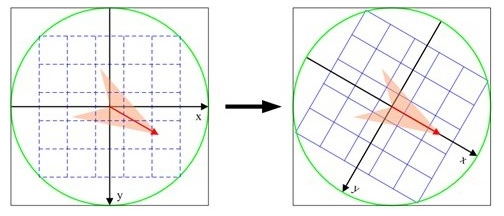
\includegraphics[width=0.5\linewidth]{yi}
\caption{将坐标移至关键点主方向}
\label{fig:yi}
\end{figure}
        
旋转后邻域内采样点的新坐标为:
\begin{align}
\left( \begin{array}{c}
x^{'} \\
y^{'} \\
\end{array} \right)
=\left( \begin{array}{cc}
\cos\sigma & -\sin\sigma \\
\sin\sigma & \cos\sigma \\
\end{array} \right)
\left( \begin{array}{c}
x \\
y \\
\end{array} \right)
\end{align}

下面就要对每个特征点求取方向直方图了,以特征点为原点,求其邻域内像素点的梯度方向直方图。梯度方向直方图是在$0\sim360$度的范围内,通常平均分为8等份,直方图中每一份是45度的范围。以特征点为中心,其周围$16\times16$的邻域内,计算每一个像素的梯度,看其梯度方向在哪一个度数范围内,直方图中就给相应的那一份加上一个权重,这里的权重就是每个像素梯度的大小。将$16\times16$的邻域再分为$4\times4$个区域,每个区域中有16个像素点,计算每个区域的梯度方向直方图,如图~\ref{fig: 128dimension}所示。这样对每个特征点就得到一个$4\times4\times8 = 128$维的特征描述子。
\begin{figure}
\centering
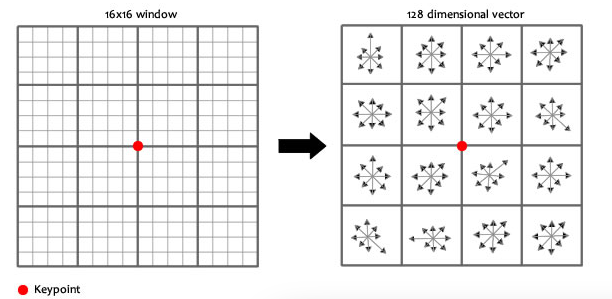
\includegraphics[width=0.5\linewidth]{sift2}
\caption{描述子用128维向量表征}
\label{fig: 128dimension}
\end{figure}

再以特征点为原点,求其邻域内像素点的梯度方向直方图。梯度方向直方图是在$0\sim360$度的范围内,通常平均分为8等份,直方图中每一份是45度的范围。假设邻域范围为$16\times16$,计算其中每一个像素的梯度,看其梯度方向在哪一个度数范围内,直方图中就给相应的那一份加上一个权重,这里的权重就是每个像素梯度的大小与高斯权重的乘积。

当邻域范围为$16\times16$时,我们通常将其又分为$4 \times 4$个区域,计算每一个区域中的8个方向的梯度方向直方图,即可形成一个种子点,一共可以生成16个种子点。

描述子向量元素门限化及门限化后的描述子向量规范化。

根据特征点的尺度对特征描述向量进行排序,生成最终的SIFT特征向量。
\end{enumerate}

\item 方向梯度直方图特征

方向梯度直方图~\cite{dalal2005histograms}(Histogram of Oriented Gradients,HOG)特征是由Navneet Dalal等人于2005年提出的一种特征描述子,它是一种局部特征,主要通过统计图像上局部区域内的梯度方向来构成直方图,最后将所有区域内的直方图串联而成。方向梯度直方图特征结合支持向量机分类算法生成分类器在图像识别方面取得了很好的效果,特别是在行人检测的应用中更是起到了重要作用。对方向梯度直方图进行求解的具体步骤如图~\ref{fig: shixian}。
\begin{figure}
\centering
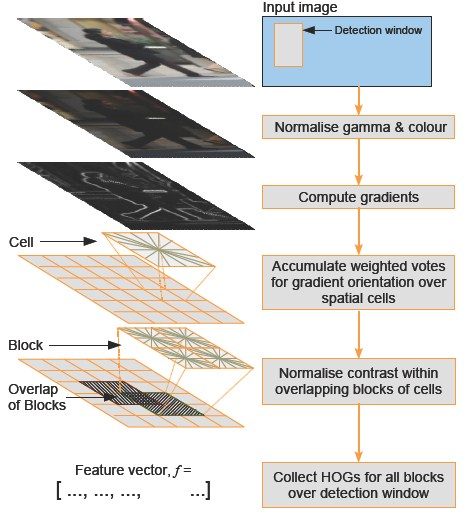
\includegraphics[width=0.4\linewidth]{flowchart}
\caption{HOG特征}
\label{fig: shixian}
\end{figure}

\begin{enumerate}
\item 首先对图像进行标准化或归一化操作。由于拍照光线不好、角度问题以及噪声等的影响,所得到的图像会有对比度低、局部昏暗等问题,对于随后的特征提取会有一定的干扰。通常采用Gamma校正法来对颜色空间进行标准化,Gamma压缩公式为:

\begin{align}
I(x,y)=I(x,y)^{gamma}
\end{align}

\item 利用一阶微分计算每一个像素的梯度(包括大小和方向),梯度方向同时也表示了目标物体的轮廓边界方向。
    
采用模板$[-1~0~1]$计算水平和垂直方向的梯度:
\begin{align}
G_{h}(x,y)=f(x+1,y)-f(x-1,y)~~~~\forall x,y\\
G_{v}(x,y)=f(x,y+1)-f(x,y-1)~~~~\forall x,y
\end{align}
        
梯度值和梯度方向的计算如下:
\begin{align}
M(x,y)=\sqrt{G_{h}(x,y)^{2}+G_{v}(x,y)^2}\\
\theta(x,y)=\arctan\frac{G_{h}(x,y)}{G_{v}(x,y)}
\end{align}
        
\item 将图像划分成小的单元(cell)(例如$6 \times 6$像素/单元)。

\item 统计每个单元内所有像素点的梯度直方图,将其作为每个单元的描述子。首先将梯度方向分为$m$份(共360度),如果分为了16份(如图~\ref{fig: bin}),则每一份中是22.5度。然后看每个像素点的梯度方向是落在了哪一份中,对应直方图中的那一份就加上一个权值,这里的权值就是像素点的梯度大小。
\begin{figure}
\centering
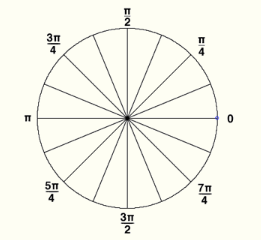
\includegraphics[width=0.3\linewidth]{bin}
\caption{梯度方向bin}
\label{fig: bin}
\end{figure}
       
\item 相邻的几个单元可以组成一个更大的块(block)(例如$3 \times 3 $个cell/block),再将一个块内所有单元的梯度直方图串联起来,最后得到该块的方向梯度直方图特征描述子。在将单元组合成块时,块与块之间是可以有重合的,这样,每个单元的梯度直方图都会被多次使用,以串联生成块的梯度直方图特征。其中块既可以按矩形划分(R-HOG),也可以按环形划分(C-HOG),具体见图~\ref{fig:shape}。
    
\begin{figure}
\centering
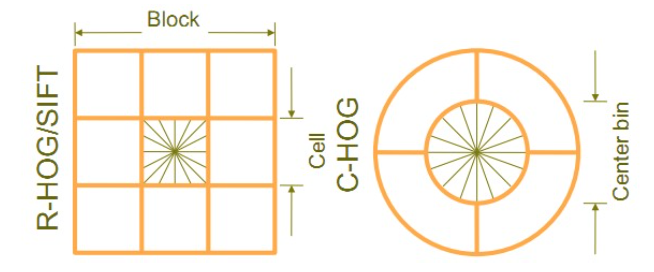
\includegraphics[width=0.5\linewidth]{shape}
\caption{矩形区间和环形区间}
\label{fig:shape}
\end{figure}
        
\item 将图像内的所有块的梯度方向直方图特征串联起来就可以得到整幅图像的梯度方向直方图特征描述子了,这个就是最终的可供分类使用的特征向量。该向量的维数为$m \times n \times \alpha$,其中$m$表示每个单元中方向bin的数目,$n$、$\alpha$分别表示块的个数以及一个块中的单元数目。
\end{enumerate}

\item SURF

SURF与SIFT算法相似,其优点是运算简单,效率高,缺点是不够稳定,并且检测出的特征点数目少一些。

算法步骤如下:

\begin{enumerate}
\item 构建Hessian矩阵。采用的是Hessian矩阵行列式近似值图像。

\item 构造多尺度空间。

构造对尺度空间的目的是实现尺度不变性,SURF算法则用高斯滤波与Hessian矩阵结合近似实现多尺度空间,计算复杂度比SIFT低。

\item 根据非极大值抑制初步确定特征点。

\item 主方向确定

\item 构造特征点算术描述子,SURF算法是选取一个20S(单位)的区域,分成$4 \times 4$分,每一份中有$5 \times 5$S,统计一份中的$\sum d_{x}$,$\sum d_{y}$,$\sum |d_{x}|$,$\sum |d_{y}|$,这样就得到$4 \times 4 \times 4 = 64$的向量描述子。SIFT是128个描述子,比SURF复杂一点。
\end{enumerate}

\item 局部二值模式特征

局部二值模式(Local Binary Pattern,LBP)~\cite{ojala1994performance}是一种用来表征图像局部纹理特征的描述子,具有旋转不变性和灰度不变性等优点。
 
 对图像中的某个像素点计算其局部二值模式值的步骤如下:以该像素点为中心,将其灰度值与其周围$3\times3$窗口的邻域内的8个像素点进行大小比较,如果邻域内像素的灰度值大于中心点的灰度值,则该邻域内像素点的值被置为1,否则置为0。经过这一阈值处理后,对每一个像素点,就得到了其邻域8个像素点的二进制表示(方向是从左上方的像素点开始往右顺时针走),再求出该二进制数的十进制表示,这就是该中心像素点上的局部二值模式值,如图~\ref{fig: lbp}。
\begin{figure}[!ht]
\centering
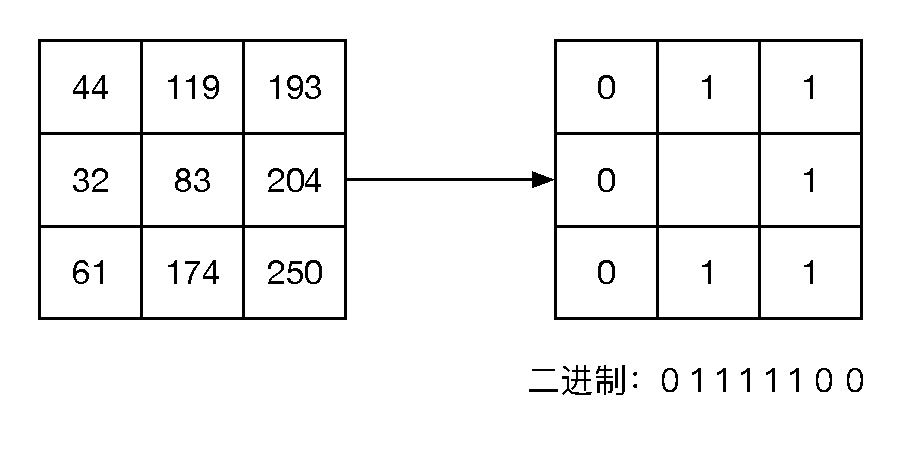
\includegraphics[width=4in]{lbpbinary.eps}
\caption{LBP特征}
\label{fig: lbp}
\end{figure}

\item FV(Fisher vector)
   
Fisher vector本质上是用似然函数的梯度vector来表达一幅图像。主要思路是用生成式模型(GMM)对样本输入进行建模,进而得到样本的一种表示(fisher vector),再将这种表示(fisher vector)输入判别式分类器(SVM)得到图像分类结果。fisher vector是fisher kernel中对样本特征的一种表示,它把一幅图片表示成一个向量。在高斯分布的基础上再找到变化的方向,可以更加准确的表示这一张图。

\item 骨架特征

骨架又称为中轴,它的定义来自于烧草模型和最大圆盘模型。骨架不仅包含了物体的几何特征,也描述了物体的拓扑结构。经典的骨架化算法有中轴变换、细化算法、Voronoi图算法等。在骨架的基础上可以通过奇点图、骨架树等对物体的结构特征进行描述。

骨架树:将骨架映射到一个树状结构(如图~\ref{fig: skeleton-tree})。骨架上的点可以分为三种类别:分叉点、端点和连接点。其中当骨架点的邻接点的数目为1时被称为端点,邻接点数目为2个或2个以上时被称为分叉点,除此之外的点被称为连接点。
\begin{figure}
\centering
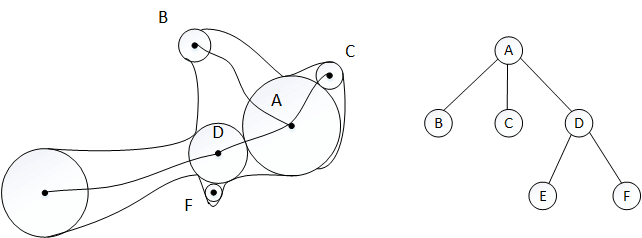
\includegraphics[width=0.6\linewidth]{skeleton-tree.png}
\caption{骨架树}
\label{fig: skeleton-tree}
\end{figure}
根据骨架树深度优先搜索产生的节点序列中的所有节点用其孩子数替换,替换后得到的新序列即为树描述符。例如,图~\ref{fig: skeleton-tree}的树描述符为(3,2,0,0,0,0)。

\item 形状上下文特征
    
    形状上下文(Shape Context, SC)由Belongie等人~\cite{belongie2002shape}提出,是基于物体轮廓样本点进行描述的。下面给出形状上下文求解的具体步骤。
    首先,对一幅图像(图~\ref{fig: ShapeDescription}(a))中的目标进行边缘提取,得到结果如图~\ref{fig: ShapeDescription}(b)所示。然后将这一轮廓看作是一定数目的采样点的集合(图~\ref{fig: ShapeDescription}(c)),利用这些采样点来描述目标形状。通过对数极坐标空间(图\ref{fig: ShapeHistogram}(a))计算每个采样点与形状其他点之间的位置关系,采用直方图表示。假设目标轮廓上采样点的集合定义为$O = \{o_1, \ldots, o_n\}$,其中$n$表示采样点的个数。假设目标轮廓是分段平滑的,当$n$充分大时,可以基本与物体实际轮廓贴合。若第$i$个采样点$o_i$作为参考坐标原点(图~\ref{fig: ShapeHistogram}(b)),建立对数极坐标映射表示剩余的$n-1$个采样点的分布情况,可以看到周围与它相邻的点(在极坐标覆盖的范围之内)落于不同的小格子内,表示不同的相对向量,这些相对向量刻画了整个形状与参考点的相对位置,因而就成为这个点的形状上下文,用直方图$h_i$表示。
\begin{align}
h_i(k) = \# \{j \ne i : (o_j - o_i) \in bin(k)\}
\label{eq: shape context}
\end{align}
以$o_i$为极坐标中心进行坐标变换,以该中心画一个圆,并把圆等分成$k$份,计算圆范围内的点落在每一份中的个数,这样对每一个点就得到一个$k$维的直方图。$\theta$为极角,$r$为极坐标半径,对于每一个由$\theta$和$logr$确定的极坐标区域,如果该区域包含的点越多,那么在由$\theta$和$logr$确定的对应形状直方图中的数值就越大。 

\begin{figure}[t]
  \centering%
  \begin{subfigure}{0.23\linewidth}
    
\includegraphics[height=3.5cm]{a1.png}
    \caption{}
  \end{subfigure}
 % \hspace{4em}%
  \begin{subfigure}{0.23\linewidth}
    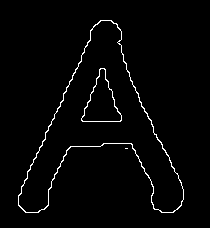
\includegraphics[height=3.5cm]{a-edge.png}
    \caption{}
  \end{subfigure}
   \begin{subfigure}{0.234\linewidth}
    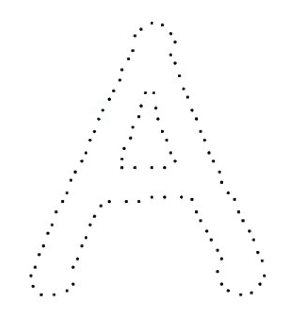
\includegraphics[height=3.5cm]{a-point.png}
    \caption{}
  \end{subfigure}
  \caption{形状描述}
  \label{fig: ShapeDescription}
\end{figure}

\begin{figure}[t]
  \centering%
  \begin{subfigure}{0.3\linewidth}
    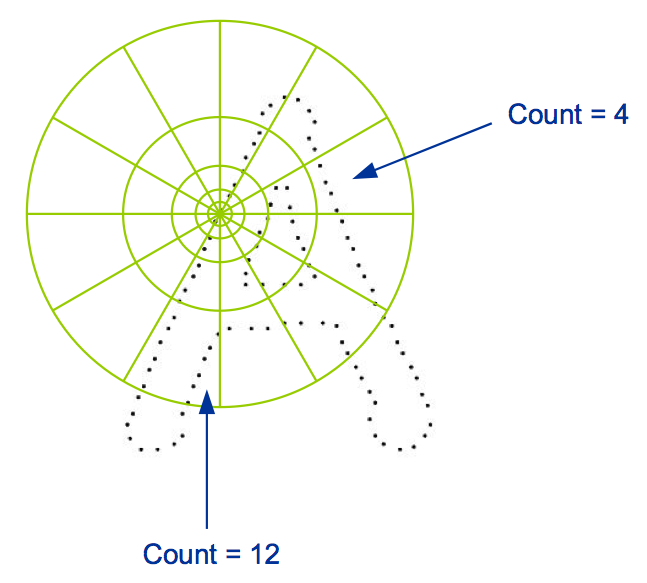
\includegraphics[height=4cm]{a-log.png}
    \caption{}
  \end{subfigure}
  \hspace{4em}%
  \begin{subfigure}{0.35\linewidth}
    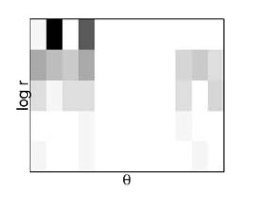
\includegraphics[height=4cm]{his.png}
    \caption{}
  \end{subfigure}
  \caption{形状上下文的直方图表示}
  \label{fig: ShapeHistogram}
\end{figure}


只要每个点的形状上下文出来了,那么对所有点的形状上下文组合起来就可以形成整个物体的形状上下文了。

在物体分类识别的应用中,是这样利用形状上下文特征的:首先对图像数据集中的每一类别都找一幅模板图像,该模板能较好地反应其所属类别图像的共性。假设对一幅图像的物体轮廓采样了100个点,就得到一个$100\times k$的矩阵。同样,对模板也能得到一个$100\times k$的矩阵。再计算图像中的每个点与模板中的每个点的距离,得到图像中的点和模板中的点的一一对应关系,结果是一个$100\times100$的矩阵。最后根据这个一一对应关系计算出一个值,表示该图像和模板之间的相似度。计算出每幅图像和所有类别模板之间的相似度,当做该幅图像的一个特征向量,利用分类算法进行训练,可以生成一个分类器。
\end{enumerate}

\subsection{其它特征}

\begin{enumerate}

\item 局部对称性

\begin{figure}[!ht]
 \centering
 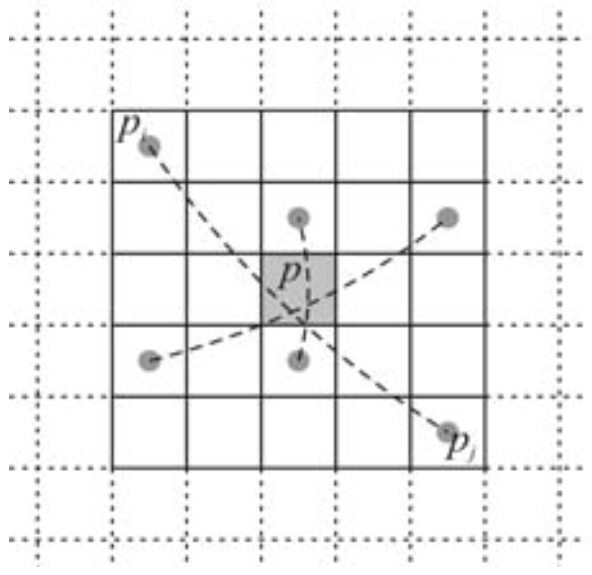
\includegraphics[width=3in]{ExamplesofPixelpairs}
\caption{用对称性算子来对像素对的梯度进行比较的三个例子}
\label{fig: ExamplesofPixelpairs}
\end{figure}

局部对称性的原理是基于周围像素的灰度梯度,计算在给定点$p$处的对称性程度。如图~\ref{fig: ExamplesofPixelpairs}所示,点$p$处的对称性可以通过比较位于$p_i$和$p_j$处的像素对$i$和$j$的灰度梯度来度量,其中$p = (p_i  = p_j)/2$。每对像素对对点$p$处的局部对称性的贡献为
\begin{align}
c(i, j) = d(i, j, \sigma) \cdot p(i, j) \cdot m_i \cdot m_j
\end{align}
$m_i$是像素点$i$的梯度的模,$d(i, j, \sigma)$是当标准差为$\sigma$时,两个像素点间的距离的高斯加权函数,对称性
\begin{align}
p(i, j) = \Big(1-cos(\gamma_i+\gamma_j)\Big)\cdot \Big(1-cos(\gamma_i-\gamma_j)\Big)
\label{eq: SymmetryMeasurement}
\end{align}

其中,$\gamma_i = \theta_i-\alpha$,见图~\ref{fig: PixelpairContribution}。当点$p_i$、$p_j$关于点$p$对称时,$\gamma_i+\gamma_i=\pi$,式~(\ref{eq: SymmetryMeasurement})中的第一项取得最大值。如果只用第一项,会使得在直线边缘上的点取得较大的值,而这些点通常并不具有对称性。为了避免这个问题,又加入了第二项,表示具有相似梯度方向的像素对。最后,对所有像素对的贡献进行求和得到点$p$处的isotropic symmetry值
\begin{align}
M^{iso}(x, y) = \sum_{(i, j)\in \Gamma(p)} c(i, j)
\label{eq: IsotropicSymmetry}
\end{align}

\begin{figure}[!ht]
 \centering
 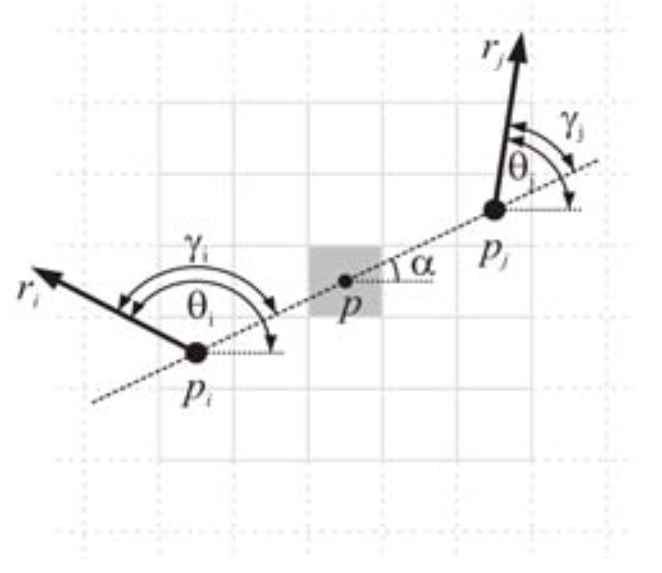
\includegraphics[width=3in]{PixelpairContribution}
\caption{每对像素对的贡献的几何表示}
\label{fig: PixelpairContribution}
\end{figure}

为了使symmetry operator对有多个对称轴的对称图案更敏感,Reisfeld等人~\cite{reisfeld1995context}又提出了radial symmetry operator,作为isotropic symmetry operator的扩展。首先,像素对的贡献的方向用$\varphi(i, j) = (\theta_i+\theta_j)/2$来计算。然后,对最大贡献为$c(i, j)$的像素对$(i, j)$,对称方向被确定为$\phi(p) = \varphi(i, j)$。这个值也用来提升有不相似方向的像素对的贡献。
\begin{align}
M^{rad}= \sum_{(i, j)\in \Gamma(p)} c(i, j) \cdot sin^2(\varphi(i, j) - \phi(p))
\end{align}

\item 灰度直方图

灰度直方图是针对灰度图像的,如果是彩色图像,可以求取其颜色直方图。若灰度级的范围为$0 \sim 255$,则灰度直方图表示这256个灰度值中的每一个在图像中出现的个数。
\end{enumerate}

\section{特征选择}

~\ref{2.3.3}和~\ref{3.1}节的介绍中基本涵盖了近年来图像处理和机器视觉领域常用的一些特征,其中有些特征适用于浮游动物图像的分类问题,有些并不适用,要对这些特征进行筛选。本文中的特征选择过程是通过对单个特征及特征组合的理论分析与实验结合,判断一个特征或一组特征对浮游动物图像分类效果的影响。其中实验部分是对~\ref{2.1}节中介绍的包含13类浮游动物的数据集分别用两种基本的分类算法(支持向量机和随机森林)进行分类,对分类结果利用$K$折交叉验证方法进行评价,看在数据集上的分类准确率和错误率有没有分别提高和降低。

对前面所总结的所有特征进行实验,我们最终选择了三类特征:PkID中用到的特征、LBP特征以及内距离形状上下文特征。相对于其它特征而言,这三类特征在对浮游动物图像的分类上效果较好,其中PkID中用到的特征数目较多,可对其进行进一步筛选。

\subsection{PkID中的22个特征}

由~\ref{2.3.3}节可以看到,PkID中共采用了67个特征,分为6大类:位置特征、尺寸特征、灰度特征、形状特征、生物统计特征和自定义特征。这些特征都是带有一定意义的,通过实验和分析,我们得出结论:位置特征不能表征浮游动物的属性,会降低分类准确率。而由于我们采用的数据集是经过扫描得到的,不同浮游动物类别有透明和不透明之分,表现在扫描图像上就是灰度值高和灰度值低,因而灰度特征可作为浮游动物图像分类的一个重要特征。由于数据集中对每幅图像都做了标尺,不同类别的浮游动物在尺寸上应该是互不相同的,但由于处于不同成长期的浮游动物以及拍摄角度(正面和侧面)的影响,会使得尺寸特征失去了本应有的效果。形状特征是表征一类物体的较为重要的特征,对于不同种类有一定的区分度。生物统计特征近年来在分类识别中使用的也比较多,效果较好,但其物理意义不是十分明确,难以从理论上说明其有用的原因,只能从实验结果上反应。

\begin{table}[ht]
\centering
\caption{对PkID中的6类特征用支持向量机和随机森林方法进行分类的分类准确率}
\begin{tabular}{|c|c|c|}
\hline
& 支持向量机 & 随机森林 \\
\hline
位置特征 & 15.3\% & 30.23\% \\
\hline
尺寸特征 & 26.04\% & 56.95\% \\
\hline
灰度特征 & 37.6\% & 61.3\% \\
\hline
形状特征 & 37\% & 63.1\% \\
\hline
生物统计特征 & 52.4\% & 69.9\% \\ 
\hline
自定义特征 & 68.05\% & 69.03\% \\
\hline
\end{tabular}
\label{PkID-6}
\end{table}

我们对这6类特征分别用支持向量机和随机森林分类算法进行实验,得到的分类准确率如表~\ref{PkID-6}所示。效果比较好的是灰度特征、形状特征、生物统计特征和自定义特征,基本符合我们对于特征的分析,从而可以将位置特征和尺寸特征筛除掉。对剩下的4类特征进行进一步实验,不断地挑选一定数量的特征,用支持向量机和随机森林分类算法进行验证,最终我们从67个PkID特征中挑出了22个,如表~\ref{表2}所示,可以看到只选取了生物统计特征、形状特征、自定义特征三种,其中一部分自定义特征是根据其他几类特征来自定义产生的,所以这里没有选取灰度特征,分类效果依然很好。

\begin{table}[htbp]
\centering
\caption{PkID中的22个特征}
\begin{tabular}{|c|l|}
\hline
生物统计特征 & Mean、StdDev、Skew、Kurt、CV、SR \\
\hline
形状特征 & Fractal、Skelarea、Circ、Symetrieh、Symetriev、Symetriehc、\\
 & Symetrievc、Elongation2、Circexc、Convperim、Convarea\\ 
 \hline
自定义特征 & MeanPos、PerimAreaexc、FeretAreaexc、PerimFeret、CDexc \\
\hline
\end{tabular}
\label{表2}
\end{table}

\subsection{局部二值模式}

   
对LBP特征向量进行提取的步骤:
\begin{enumerate}
    \item 首先将检测窗口划分为$16\times16$的单元(cell)。
    \item 对于每个单元中的一个像素,将相邻的8个像素的灰度值与其进行比较,若周围像素值大于中心像素值,则该像素点的位置被标记为1,否则为0。这样,$3\times3$邻域内的8个点经比较可产生8位二进制数,即得到该窗口中心像素点的LBP值。
    \item 然后计算每个单元的LBP值直方图,即每个数字(假定是十进制数LBP值)出现的频率,然后对该直方图进行归一化处理。
    \item 最后将得到的每个单元的统计直方图进行连接成为一个特征向量,也就是整幅图的LBP纹理特征向量。
\end{enumerate}

\subsection{内距离形状上下文}

本文~\ref{2.3.2}节中介绍了关于形状上下文的内容,由于形状上下文不能很好地解决物体类内部之间的变形,后期产生了改进的基于内部距离的形状上下文~\cite{ling2007shape},内距离形状上下文中采用内距离代替欧式距离。

采用内距离形状上下文提取图像特征的基本步骤如下:
\begin{enumerate}
\item 先从图像中挑选$m\times n$张图像作为模板(每类浮游动物中选取$m$张,共$n$类)。
\item 采用内距离形状上下文分别计算训练集和测试集中所有图像和上一步骤中$m\times n$张图像间的距离。
\item 将上面计算得到的距离矩阵作为训练集和测试集的特征,输入到ELM中进行学习和分类。
\end{enumerate}
